% 2
%\documentclass[comp]{icu} % 提出用のフォーマット
\documentclass{jsbook}
%\usepackage[dvips]{graphicx}
\usepackage[dvipdfmx]{graphicx}
\usepackage{amsmath,amssymb}
\usepackage{verbatim}

%==== タイトル部分
%\title{タイトル}
%\題名{日本語の題名}
%\author{SUZUKI, Nanigashi}
%\氏名{鈴木 某}
%\date{March, 2002} % 自分の卒業する時期は自分で書き込もう
%==== タイトル定義ここまで

\begin{document}
%\maketitle % これで中表紙ができる
%\frontmatter
%\tableofcontents\newpage
%\listoftables\listoffigures
%\input{acknowledgment}
%\mainmatter
\setlength{\baselineskip}{2em} % 行間の自動調整を停止したので
                               % 本文の直前にこの1行を加えて対処をお願いします
\setcounter{chapter}{1}
\chapter{統計学習 (Statistical Learning)}
\section{統計学習って何?}
何故そもそも統計なんて勉強するのか?Figure 2.1を見てほしい。

X軸はそれぞれTV、radio、新聞の広告予算であり、Y軸は
ある商品の売上金額である。
企業にとって売上を伸ばすことが重要課題であるが、
それらは直接コントロールできない。
その代わりに、広告を打ち出すことで間接的に
売上をコントロールすることができる。
どれくらい広告を打ち出せば、達成すべき売上に到達できるのか、
そのモデルを与えるのが統計であり、企業の意思決定に必要なものである。


%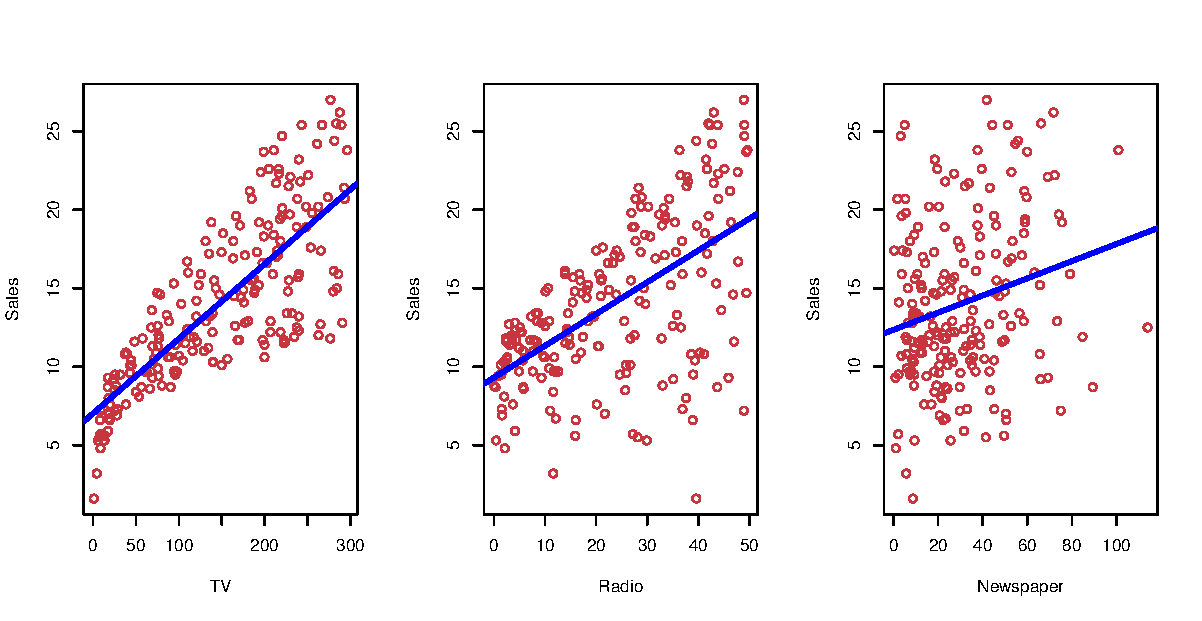
\includegraphics[width=5cm,clip]{fig_2/2.1.pdf}


ここで、言葉の整理をしておく。
\begin{itemize}
\item 広告量:入力変数、もしくは説明変数($X_1, X_2, \cdots$)
\item 売上:目的変数、もしくは被説明変数($Y$と表す)
\end{itemize}

より一般的に、連続的な値をとる目的変数$Y$と$p$個の異なる
説明変数($X_1, \cdots, X_p$)に、ある種の関係性があるとすると、
\begin{equation}
  Y = f(X) + \varepsilon
\end{equation}
と表せる。ここで、$f$は固定された、しかし未知の関数であり、
$\varepsilon$は誤差項である。

別の例として、年収と教育年月との関係性を持つデータを紹介する。
FIgure 2.2には、$x$軸に教育年数、$y$軸に年収をとり、30人の
データを示している(ただし、実際のデータではなくシミュレーションデータ)。
シミュレーションデータなので、どのような関数$f$を用いているか
既知である(Figure 2.2右の青い線)が、一般的に$f$の形は不明である。
基本的には、データの分布を見て決定するのが1つの方法としてある。

より一般的には、関数$f$は多数の説明変数を入力値として持つ。
Figure 2.3に年収を教育年数と、勤続件数の2つの説明変数を用いて
予測するモデル結果を示している。

基本的に、統計学習は、$f$を算出するためのアプローチのことだと思ってくれればよい。

\subsection{なぜ$f$を算出するのか?}
目的は大別すると2つある:予測と推定。以下、それぞれについて説明する。

\subsubsection{予測}
よくある状況として、説明変数$X$は簡単に得られるが、
被説明変数$Y$は簡単に得られない場合が多い。
そんな時、$f$がわかっていると、
\begin{equation}
	\hat{Y} = \hat{f}(X)
\end{equation}
で被説明変数$Y$を求めることができる。(平均すると、誤差項は0という分布を
仮定したので、上の式には誤差項はない。)
また、ここで$\hat{Y}$や$\hat{f}$は、我々が分析した推定値である。
このような場合、$\hat{Y}$さえわかれば良いという考えが往々にしてあるので、
$\hat{f}$はブラックボックスでも構わない。

さて、予測が(実測値と比較して)どれくらいの精度でできるのか?
その精度は2つの量により定義される:reducible errorとirreducible error。
一般に、関数$f$の形や、パラメータはわからないので、
データから$f$を特定したとしても、実際の$f$と異なる可能性が十分ある。
その差異がreducible errorと呼ばれる。
reducible(小さくすることができる)と名前がつけられているのは、
もし関数$f$を実際の$f$と同じ関数形に算出することができれば、
関数$f$と$\hat{f}$の差はゼロにすることができるからである:
$$
	|\hat{f} - f| \sim 0
$$
しかし、実際の値は関数$f$だけでなく、誤差項$\varepsilon$も含んでいるので、
$$
	|\hat{Y} - Y| \sim \varepsilon \hspace{5mm} (\text{when}  \hat{f} = f)
$$
と分析者がどうしても誤差項を小さくすることはできない。これがirreducible error(
どんなに頑張っても小さく出来ない誤差項)である。

以上の議論を定量的に扱ってみる。 実測値と予測値の差の2乗の平均は、
\begin{eqnarray}
\lefteqn{E[(Y - \hat{Y})^2]} \nonumber \\ 
		& = & E[(f(X) + \varepsilon - \hat{f}(X))^2]  \hspace{1cm}  \nonumber \\ 
		& = & E[ a + \varepsilon ]^2 \hspace{1cm} (a = f(X) - \hat{f}(X)) \nonumber \\
		& = & E[ a^2 + 2 a \varepsilon + \varepsilon^2] \nonumber \\
		& = & E[ a^2 ] + \text{Var}(\varepsilon) \hspace{1cm} (E[x+y] = E[x] + E[y], E[\varepsilon^2] = \text{Var}(\varepsilon)) \nonumber \\
		& = & E[ ( f(X) - \hat{f}(X))^2 ] + \text{Var}(\varepsilon) \nonumber \\
		& = & [f(X) - \hat{f}(X)]^2 + \text{Var}(\varepsilon). \label{2:eq diff1}
\end{eqnarray}
となり、前の項がreducible error、後ろの項がirreducible errorである。

この本では、(後ろの項はどうしようもないので)reducible errorを最小にするような
$f$を算出することを目的とする。
ただし、気をつけないといけないのは、予測誤差の下限値(一番良い誤差)は
irreducibleで定義されており、これはどうしようもないし、
さらには、どれくらいirreducible errorの大きさを持つのかも一般的にはわからない。

\subsubsection{推定(Inference)}
推定の目的は、被説明変数に対する、各々の説明変数の影響度合いを調べることである。
(例:TV広告出稿を10%増加させると、売上が2%上昇する)。
このとき、予測の時で許されたブラックボックス$f$は許されないことが多い。

\subsection{$f$の算出方法}
以降の章で、$f$について色々な手法を紹介するが、
共通する部分もあるので、ここで取り上げる。
以降、データで$n$観測点があるとする。また、説明変数は$p$個あるとして、
トレーニングデータセットは、$\{(x_1, y_1), (x_2, y_2), \cdots, (x_n, y_n)\}$、
ここで$x_i = (x_{i1}, x_{i2}, \cdots, x_{ip})^T$である。

\subsubsection{パラメトリックな手法}
パラメトリックな手法は以下の2ステップで構成される。
\begin{enumerate}
\item $f$の関数形を決める。例えば、$X$に対して線形だと仮定すると、
	\begin{equation}
		f(X) = \beta_0 + \beta_1 X_1 + \beta_2 X_2 + \cdots + \beta_p X_p.
	\end{equation}
	$f$の形を決めてしまえば、問題はものすごく単純になる。すなわち、
	もともと$p$個の引数をとる$f(X)$を求めることから、
	$p+1$個の係数$\beta_0, \beta_1, \cdots, \beta_p$を算出することに置き換わる。
\item 関数形を決めた後、トレーニングデータに合わせるようパラメータを決定する。
	上の例だと、$\beta_0, \beta_1, \cdots, \beta_p$を求めることに等しい。
	よく使われる手法に、(ordinary) least squaresがある(3章でやる)。
	それ以外にもたくさん手法があるが、それは6章で紹介する。
\end{enumerate}
ここで紹介した方法がパラメトリックな手法と言われるもので、
$f$を算出する問題を、幾つかのパラメータを算出する問題に置き換えていることに由来する。

パラメトリックな手法は問題を簡単にする分、別の問題が生じる。
\begin{itemize}
\item もし、本当の関数形(わかる分けないが)と異なる関数形を決定してしまうと、
reducible errorが大きくなる。
\item パラメータ数をとてつもなく大きくして、関数が柔軟な形をとるようにもできるが、
今度は、トレーニングデータに合わせすぎてしまい、テストデータと予測値が
全然合わないことがおきてしまう(過学習、オーバートレーニング)。
\end{itemize}

Figure 2.4に、年収を目的変数に、教育と勤続年数を説明変数とした予測値と、実測値を示す。
関数形は以下の式で与えられる。
$$
	(income) \sim \beta_0 + \beta_1 \times (education) + \beta_2 \times (seniority)
$$

\subsubsection{ノンパラメトリックな手法}
ノンパラメトリックな手法は、関数の形を最初に決めない。
そうすることで、真の関数形$f$と全く異なるという危険性は回避できる。
しかし、$f$を算出することを幾つかのパラメータを求める、という問題の単純化を
行っていないので、データ数$n$は十分大きいことが求められる。

Figure 2.5にノンパラメトリック手法の1つのthin-plate splineで求めたモデルを示す。
Figure 2.3が真の関数形であるが、それとほぼ同じことがわかる。
スプライン関数を使用するとき、関数形がどれくらいスムーズなのか、分析者は
入力する必要がある。
Figure 2.6にスムーズ性をほぼなくした結果を示す。
トレーニングデータと予測値の誤差が0となっていることがわかり、
オーバートレーニングしていることが読み取れる。

どういう風にスムーズ性を入れればよいのかは5章で、
スプライン関数については7章で述べる。

\subsection{予測精度と解釈可能性のトレードオフ}
線形回帰モデルの場合、関数の形を事前に決めてしまうため、
柔軟性に欠ける。一方、ノンパラメトリックな手法のところで示した、
スプライン関数による回帰は、柔軟に$f$を決定できるため、柔軟性がある。

しかし、柔軟性に欠ける線形回帰モデルは、意味の解釈は容易である。
反対に、スプライン関数において説明変数と被説明変数の関係性を
言及しようとすると、難しい。

Figure 2.7に柔軟性を$x$軸に、解釈可能性を$y$軸にとり、
様々なモデルをその中に示した。
線形回帰(Lease Squares)よりも解釈可能性が高いものに、
Lasso回帰モデルがあるが、これについては6章で詳細に述べる。
Lasso回帰は、単純に説明すると、Least Squaresで見積もった
回帰係数$\beta_0, \beta_1, \cdots, \beta_p$のうち、いくつかは0となり、
パラメータの個数が小さくなるというものである。すなわち、
$$
	f(X) = \beta_0^{\prime} + \beta_1^{\prime} X_1 + \cdots \beta_m^{\prime} X_m \hspace{3mm}(where \hspace{2mm} m \le p).
$$
Generalized addtive models (GAMs)は7章で説明するが、線形モデルに、
ある非線形関係を許すものである。
bagging, boosting, support vector machinesは8、9章で説明するが
柔軟性は高いが、解釈は難しい。

\subsection{教師つき vs. 教師なし学習}
\begin{itemize}
\item 教師つき学習:線形回帰、ロジスティック回帰、GAM、boosting、SVM
\item 教師なし学習:クラスター分析 or クラスタリングなど(詳細は10章)
\end{itemize}
Figure 2.8はクラスター分析の結果を示している。
説明変数は2つしかないので、散布図を描くのは容易だが、
説明変数が$p$個あると、組み合わせは$p(p-1)/2$個となり、
散布図を描くのも困難になる。
この辺りも10章で述べる。

また、教師つきか、教師なしか問題がはっきりしないこともある。
例えば、$n$個のデータのうち$m$個のみが説明変数と被説明変数両方の
値を持っていて、$n-m$個が説明変数のみ値を持っているという場合がある。
こういう問題はsemi-supervised learning 問題と呼ばれる。
望むべきは、$m$個のデータと、$n-m$個のデータを全て学習させることが
できる方法があればいいが、この話題は本書のスコープ外である。

\subsection{回帰 vs. 分類問題}
ひとまず、以下のように認識してもらえば問題ない。
\begin{itemize}
\item 回帰:被説明変数が連続値をとる
\item 分類:被説明変数が離散値をとる
\end{itemize}

\section{モデル精度の評価(Assessing Model Accuracy)}
この節では、あるデータが与えられた際に
どの統計モデルを選択するか、という事について概念的に述べる。
(具体的な例は後の章でやります。たぶん。)

\subsection{フィッティング精度の測定}
統計モデル$f$が与えられたとき、どれくらいデータにフィットされているのかを
議論したい。
回帰の場合、よく平均2乗誤差(mean squared error, MSE)
\begin{equation}
MSE = \frac{1}{n} \sum_{i=1}^n (y_i - \hat{f}(x_i))^2 \label{2:eq MSEtrain}
\end{equation}
が用いられる。ここで$\hat{f}(x_i)$は$i$番目の観測量における予測値である。
もちろん、MSEが小さいほどデータをよく再現できているということになる。

(これから述べることは超重要なので、記憶しておいてください。)
式~\eqref{2:eq MSEtrain} はモデル$f$に対してフィッティングさせた、
トレーニングデータに対して計算しているので、正確には
training MSEと呼ばれる。
しかし、一般的には、分析者はトレーニングデータの精度はあまり気にしないことが多く、
むしろ興味があるのは、未知のデータが入ってきたとき、どれくらい精度よく
予測できるのだろうか、ということである(未知のテストデータ、あるいは誤解がないときは
単にテストデータと呼ばれることもある)。
例をあげると、
\begin{itemize}
\item 天気予報を過去数十年のデータから、天気予報が90%あたるモデル式を構築したとしても、
果たして明日の天気が90%で予測できるのか?
\item ある会社の株価を、有効求人倍率や、鉱工業生産数などで80%の精度で予測したとしても、
果たして明日の株価が80%で予測できるのか?
\end{itemize}

数式で言ってみると以下のようになる。
トレーニングのデータセットが$n$個$\{(x_1, y_1), (x_2, y_2), \cdots, (x_n, y_n) \}$
あって、それを用いて$\hat{f}$を算出したとする。
手元には、$\hat{f}(x_1), \cdots, \hat{f}(x_n)$があって、上記の議論から、
これは小さいと仮定する(すなわち、よくデータにあうように
$f$を推定できた、という意味)。
しかし、今興味があるのは、新たに$(x_0, y_0)$というデータ(複数のデータ含む)
が手に入ったとき、どれくらい$\hat{f}$で予測できるか、ということである。
すなわち、以下の量を計算したい:
\begin{equation}
	\text{Ave}(y_0 - \hat{f}(x_0))^2.
\end{equation}
この量(test MSEと呼ぶ)を出来る限り小さくしたい。

トレーニングデータセットと、テストデータセットは共に与えられる場合があるが、
トレーニングデータセットしか得られない場合の方が多い。
そういう場合、どういう風にモデルを選択すればいいのか。
単純に考えると、training MSEを小さくするモデルを採択したくなる
(誤差が一番小さくするようなモデルを選ぶのは当然!)。
しかし、この方法は大概オーバーフィッティングしてしまいがちである
(すなわちtraining MSEは最小だけれど、test MSEは大きくなってしまう)。

Figure 2.9 に単純な例を示す。左側のグラフには、シミュレーションによって
発生させたデータ点($\circ$)と、真のモデル$f$が黒線で描かれている。
データに対してフィッティングさせた結果が他の3線で、
オレンジは線形回帰を、水色と緑色はスプライン関数でフィッティングさせたものである
(緑色の方がsmoothnessが小さい)。
右の図には、トレーニングデータとテストデータのMSEの大きさを、
柔軟性を$x$軸にとって示している。線形回帰のもの(オレンジ)が柔軟性がもっとも低く、
逆に、柔軟性が最も高い (smoothnessが小さい) スプライン関数が右側にきている。
赤色の線がテストデータ、灰色の線がトレーニングデータの値を示しており、
テストデータのMSEはトレーニングデータのMSEよりも大きくなっている。
また、柔軟性を大きくした、緑色は、トレーニングデータでのMSEは小さいが、
テストデータのMSEは極小ではないことが見て取れる。

ここで重要なのは、(何度も言うが)training MSEが極小をとるときに、
test MSEは極小とならない、ということである。
一般的に、training MSEは柔軟性が増すにつれて小さくなるが、
test MSEはU字のようになる。

Figure 2.10に真の関数形が直線の場合を、
Figure 2.11に真の関数形が波をうっているような、ギザギザな
場合をそれぞれ示している。
Figure 2.9と比べて、test MSEの極小点が左にいくか、
それとも右にいっているか、という違いだけ。

最後に、テストデータが得られない場合に、
トレーニングデータからテストデータを生成する手法があり (cross validation)、
これについては5章で述べる。

\subsection{バイアス-バリアンスのトレードオフ(The Bias-Variance Trade-Off)}
test MSEに見られたU-shapeは、統計学習において
2つの競合する性質によるものである。
数学的に導出するのは、この本のスコープ外であるが、
説明だけはしておく。

test MSEの2乗の期待値は、3つの量で定義される:
関数$\hat{f}(x_0)$のバリアンス (variance)、2乗のバイアス (squared bias)、
誤差項のバリアンス。
すなわち、
\begin{equation}
	E(y_0 - \hat{f}(x_0))^2 = \text{Var}(\hat{f}(x_0)) + [\text{Bias}(\hat{f}(x_0))]^2 + \text{Var}(\varepsilon).
\end{equation}
$E(y_0 - \hat{f}(x_0))^2$は、test MSEの期待値を意味する。すなわち、
もし何度もトレーニングデータセットと、テストデータセットが
得られる状況での、test MSEの平均ということである。
この式から、最小のtest MSEを見つけるときには、low varianceかつlow biasの
関数$\hat{f}$を算出すればよい、ということである(test MSEの下限値は irreducible error (2.3)で定義されており、
これ以上の精度の改善は見込めない)。

さて、ここでバリアンス、バイアスの意味を以下にそれぞれ述べる。
\begin{itemize}
\item バリアンス (variance)とは、もし(今使用しているものと)異なるトレーニングデータを
関数$\hat{f}$の算出に使用した場合、どれくらい変わるのか、という量。
(真のモデルが既知ならば、誤差項の影響でデータが変わった、という意味。
全く別のデータというわけではない。念のため。)
以前の例で、スムーズ性が小さいスプライン関数があったが、
もしそういう場合に別のトレーニングデータが提供されれば、
関数の形は大きく異なることが想像できるだろう。
すなわち、(柔軟性が大きい統計モデルは)大きなバリアンスをもつということである。
また、線形回帰モデルの場合、トレーニングデータが変更されても、
パラメータが少し影響を受け変更されるかもしれないが、
大きく予測値が変わる、ということもないであろう(low variance)。
\item バイアス(bias)とは、単純には算出されたモデル式$\hat{f}$と、
実測値あるいは真の関数形との差である
(真の関数形がわかっているシミュレーションの場合は真の関数形$f$、
そうでない場合はデータとの適合度みたいなもので認識しておいてください。
ここは、ちょっと細かい定義とか言い出すと、とたんに難しくなるのでフワッとぼやかしておきます)。
例えば、真のモデルが波をうったスプライン関数で、それに
線形回帰をしても、全然合わないことが想像できるだろう(high bias)。
\end{itemize}

以上から、low-varianceをとればhigh-biasに、low-biasをとればhigh-varianceに
なることが理解できるだろう。

Figure 2.12にFigure 2.9-2.11でのMSEに、BiasとVarianceを重ねて描いたものを示す。
見てわかるように、柔軟性を大きくする(すなわちbiasを小さくする)と、
varianceが大きくなる。これをbias-variance トレードオフという。

\subsection{分類における精度評価 (The Classification Setting)}
今までの議論は、回帰、すなわち目的変数が連続値をとる統計モデルに
関して述べてきたが、
分類の場合にもbias-varianceトレードオフのような事が
同じように当てはまる。
今、トレーニングデータ$\{(x_1, y_1), \cdots, (x_n, y_n)\}$があり、
$y_i$は離散的な値をとるとする。
この時、モデル$\hat{f}$の精度評価をする際、一般的なアプローチは
training error rateを以下のように定義し、それを使用する:
\begin{equation}
	\frac{1}{n}\sum_{i=1}^n I(y_i \neq \hat{y}_i).
\end{equation}
ここで、$\hat{y}_i$は$i$番目の観測値から$\hat{f}$を使った予測値である。
$I(y_i \neq \hat{y}_i))$は {\textit{indicator variable}}(インジケータ変数と日本語ではいう?)
であり、もし予測値の分類と実測値の分類があっていれば0を、間違っていれば1を返すものである。
すなわち、上の式は、$n$個のうち分類を間違っていた数を$n$で割った量であり、
誤差率と呼ぶにふさわしい。

ただ、回帰のときと同じように、正確にはtraining error rateである。
実際はtraining error rateよりもtest error rate
\begin{equation}
	\text{Ave}(I(y_0 \neq \hat{y}_0))
\end{equation}
を最小にするようなモデルが欲しい。

\subsubsection{ベイズ分類器 (The Bayes Classifier)}
数学的な証明は省くが、test errorを最小にするような分類方法は、
各クラスの確率を算出して、確率が最大となるクラスを当てるというものである。
すなわち、分類方法が$J$個あって、説明変数$x_0$が与えられた時、$j$番目のクラスになる確率
\begin{equation}
	\text{Pr}(Y = j | X = x_0) \label{2:eq cond}
\end{equation}
を算出し、確率最大となるクラスを予測値とする。
~\eqref{2:eq cond}は条件付き確率と呼ばれる(説明変数$x_0$が与えられたもとでの$j$番目のクラス
になる確率)。
この単純な分類器をベイズ分類器と呼ぶ。
よく例としてあがるのは、$J=2$、すなわち、信号かバックグラウンドかの場合で、
この時、確率が0.5以上になる方を予測値として採用する。

Figure 2.13に$J=2$の場合のシミュレーションデータを用いたベイズ分類器での分類を示す。
紫色の破線で示されているところが境界条件、すなわち、条件付き確率が0.5になる場合である。
シュミレーションデータであるので、どういう確率分布からデータが生成されているかが
この場合は既知であり、条件付き確率が計算できる。

ベイズ分類器による誤差率をベイズ誤差率と呼ぶ。
ベイズ分類器は条件付き確率が最大となる分類$j$を採択するので、
誤差率は $1- \text{max}_j Pr(Y=j | X = x_0)$ となる。
一般に、多数のテストデータが得られる場合、誤差率は平均するのがほとんどなので、
\begin{equation}
	1 - E ( \text{max}_j \text{Pr}(Y = j | X))
\end{equation}
となる。

\subsubsection{K-nearest Neighbors (K-最近傍?)}
現実問題は、条件付き確率を計算できないので、ベイズ分類器は使用不可である。
そのため、何らかの確率を計算し、それを基準にクラス分けする必要がある。
そういう方法の1つに、K-nearest neighbors (KNN)分類器がある。
これは、テストデータの説明変数$x_0$の周辺にある$K$個のトレーニングデータを
同定し、そのトレーニングデータがどの分類になっているか、多数決をとるものである。
確率としては、
\begin{equation}
	\text{Pr}(Y = j | X = x_0) = \frac{1}{K} \sum_{i \epsilon N_0} I(y_i = j)
\end{equation}
を求めて、確率最大となるクラスをテストデータに当てはめる。
ここで、$N_0$はテストデータ$x_0$の周辺にあるトレーニングデータ$K$個の集合である。

Figure 2.15に$K=10$としたKNN分類結果を示す。破線がベイズ分類器による理論値
(この場合シュミレーションデータなので、条件付き確率は算出できるため)、
実線がKNNであり、大体よく予測できているようである。

容易に想像できるように、もしテストデータの最近傍の個数$K$を1個などとしてしまうと、
テストデータが変わる度に大きくKNNの予測が変化する (high variance)。
逆に、$K$を大きくしてしまうと、今度はデータ全体でならされてしまい、
予測精度が落ちる (high bias)。
Figure 2.16にその様子が示されている。

分類の場合の柔軟性は、KNNの場合$1/K$である。
$K$の下限値はもちろん1であり、上限値は全トレーニングデータ数$N$である。
すなわち、$1/K$は$1/N \le K \le 1.0$を満たす。
回帰の場合と同様に、test error と training error を$y$軸に、
柔軟性を$x$軸にとったものを示す。
回帰と同様に、test errorがU-shapeなのが見て取れる。

\section{Lab: Introduction to R}
今のところ割愛する。

\end{document}
